% =====================================================================
%  Energy-Efficient Train Driving via Simulator-in-the-Loop Deep RL
%  JOURNAL VERSION, REVISION 2 - compiles with pdfLaTeX on Overleaf
%
%  This revision keeps every number, equation, table and reference from
%  revision 1 but rewrites the prose throughout. The TODO(author) and
%  TODO(power) comments from revision 1 still apply and are kept.
% =====================================================================
\documentclass[11pt,a4paper]{article}

\usepackage[utf8]{inputenc}
\usepackage[T1]{fontenc}
\usepackage[margin=2.5cm]{geometry}
\usepackage{graphicx}
\usepackage{amsmath,amssymb}
\usepackage{booktabs}
\usepackage{multirow}
\usepackage{threeparttable}
\usepackage{xcolor}
\usepackage{microtype}
\usepackage{authblk}
\usepackage[colorlinks=true,linkcolor=blue!60!black,citecolor=blue!60!black,urlcolor=blue!60!black]{hyperref}

\graphicspath{{figures/}}

\newcommand{\kwh}{\,kWh}

\title{Deep Reinforcement Learning for Energy-Efficient Train Operation:\\
A Simulator-in-the-Loop Study of the Tashkent--Khojikent Suburban Line}

\author[1]{Asilbek Boboyev}
\author[1]{Komil Mustaev}
\affil[1]{Department of Software Engineering, School of Computing,\\
New Uzbekistan University, Tashkent, Uzbekistan\\
\texttt{\{a.boboev, k.mustaev\}@newuu.uz}}
\date{}

\begin{document}
\maketitle

\begin{abstract}
Driving a train so that it meets its timetable on the least traction
energy is an old operational problem. Reinforcement learning (RL) can, in
principle, learn such driving directly from a simulator, with no need for
the switching-point analysis of classical optimal control. What it
actually costs to get an agent working against a realistic simulator is
rarely written down. We report that cost for one concrete case: an ER9E
electric multiple unit on the 74.9\,km Tashkent--Khojikent suburban line
in Uzbekistan. The open-source NeTrainSim simulator was rebuilt with GOST
resistance formulas, its regenerative braking was disabled because the
ER9E has none, and an interactive bridge let a proximal policy
optimization (PPO) agent set the traction notch every second. Before the
agent learned anything useful, four faults had to be found. Elevation
noise in the route data produced grades of up to $\pm17\%$ and inflated
the simulator's energy accounting roughly threefold on the affected
links. Observation scaling left over from an earlier dataset hid gradient
and power information from the policy. The schedule term in the reward
was non-Markovian because no clock appeared among the observations. And a
constant entropy bonus kept the policy stuck at the uniform distribution.
With these fixed, the agent climbs the forward direction in 6{,}417\,s on
790.0\kwh: on schedule, within about 1\kwh{} of the constant-notch Pareto
frontier, 6.9\% below the simulator's own driver, 8.4\% below
maximum-notch driving. On the descent the same recipe finds cheaper
solutions that arrive late (169.6\kwh, 8.9\% past the deadline). We trace
the lateness to an underpriced schedule term and work out the correction.
The diagnostic procedure, more than the final policy, is what we expect
to transfer to other simulator-in-the-loop RL problems.

\medskip
\noindent\textbf{Keywords:} energy-efficient train control; deep
reinforcement learning; proximal policy optimization; railway simulation;
NeTrainSim; eco-driving; suburban railway
\end{abstract}

% =====================================================================
\section{Introduction}
\label{sec:intro}
% =====================================================================

Electric traction is a large item in railway operating budgets and, in
several countries, a noticeable share of national electricity demand. For
a train running a fixed route against a fixed timetable, the driver's use
of the throttle is one of the few levers left for saving energy. Between
the fastest feasible trip and the slowest one that still meets the
schedule there is an energy--time trade-off, and a skilled driver, or an
automatic train operation (ATO) system, can sit on the cheap end of
it~\cite{scheepmaker2017,howlett1995,yin2017}. The classical treatment
poses this as an optimal-control problem and derives a sequence of
driving regimes, typically full power, cruising, coasting, and
braking~\cite{liu2003,albrecht2016}. Deep RL offers a different route.
Given a faithful simulator of the train and the line, an agent can learn
its driving policy from interaction alone. No switching points need to be
derived by hand, and the policy can in principle respond to terrain,
speed-limit structure, and schedule slack at the same time.

This paper reports what it took to build such a system for one regional
case: the Tashkent--Khojikent (Uzbek: Toshkent--Xo\textquotesingle
jakent) suburban line, 74.9\,km long, with speed zones between 40 and
80\,km/h and a net climb of 347\,m, worked by an ER9E electric multiple
unit. We did not plan to spend most of the project on data and reward
debugging, but that is where the time went, and we believe the debugging
itself is the most useful part to publish. The contributions are the
following.

\begin{enumerate}
  \item A simulator-in-the-loop RL pipeline. We extend the open-source
  NeTrainSim freight simulator~\cite{aredah2024} in three ways:
  GOST-based resistance physics suitable for the region, removal of
  regenerative braking to match the rolling stock, and an interactive
  stdin/stdout JSON protocol through which a Gymnasium environment drives
  the C++ physics one second at a time, bypassing the simulator's
  built-in driver and optimizer.

  \item Repair of the route data. The digital elevation model behind the
  route contained single-node errors that produced grades of up to
  $\pm17\%$ on 50\,m segments. No real railway is built like that. The
  spikes broke the simulator's force balance and inflated its energy
  accounting by roughly a factor of three on the affected links. We
  repair the elevation profile with a median filter that preserves the
  net climb exactly and re-measure every baseline on the cleaned data
  (Section~\ref{sec:data}).

  \item A diagnostic chain that others can reuse. Four distinct failure
  modes stood between us and a working agent: saturated observations, a
  schedule reward that was non-Markovian, a deadlock between exploration
  and commitment under a constant entropy bonus, and lateness that was
  priced too cheaply. Section~\ref{sec:results} documents each one
  together with the measurement that exposed it.

  \item Quantified results in both directions. The final forward-trip
  policy reaches the constant-notch energy--time Pareto frontier on
  schedule (790.0\kwh{} in 6{,}417\,s), beating the simulator's native
  driver by 6.9\% and maximum-notch driving by 8.4\%. On the descending
  return trip the same procedure converges to very low energy
  (169.6\kwh) but misses the deadline by 8.9\%, which pins the remaining
  open problem on reward calibration rather than on the optimizer
  (Section~\ref{sec:discussion}).
\end{enumerate}

We are equally explicit about what the agent does not do. It matches the
constant-notch frontier; it does not move below it. And its greedy
(argmax) mode settles one notch under the schedule-feasible optimum on
both trips. Both shortcomings have a quantitative explanation, and both
have a concrete remedy.

The paper proceeds as follows. Section~\ref{sec:related} reviews prior
work on energy-efficient train control and on learning-based driving.
Section~\ref{sec:methods} covers the simulation platform, the route data
and its repair, and the Markov decision process (MDP) formulation.
Section~\ref{sec:results} gives the baselines, the diagnostic chain, and
the learning results for both directions. Section~\ref{sec:discussion}
draws out the general lessons and the limitations, and
Section~\ref{sec:conclusion} concludes.

% =====================================================================
\section{Related Work}
\label{sec:related}
% =====================================================================

\paragraph{Optimal train control.} Energy-efficient driving has been
treated as an optimal-control problem since the 1960s. Scheepmaker et
al.~\cite{scheepmaker2017} survey the field; Yin et al.~\cite{yin2017}
survey it from the ATO side. Pontryagin-type analyses show that on level
track the optimal regime sequence is full acceleration, cruising
(possibly at partial power), coasting, then full
braking~\cite{howlett1995,liu2003}, and the main results carry over to
varying gradients and speed restrictions~\cite{albrecht2016}. All of
these methods need an explicit, differentiable model of the train, and
their output is a set of switching points along the line.

\paragraph{Learning-based train driving.} RL entered the field as a
model-free alternative, first with tabular and expert-augmented methods
for metro systems~\cite{yin2014}, then, after deep RL became
practical~\cite{mnih2015}, with neural policies for speed-profile
tracking and energy reduction. Most published studies run against
simplified train dynamics written in Python for the purpose. Work that
couples a learning agent to an established, independently validated
simulator at every control step is comparatively rare. That is the
approach we take, and in our experience the coupling itself, meaning data
quality, observation design, and reward calibration against the
simulator's own accounting, is where most of the practical difficulty
lives.

\paragraph{Simulation platforms.} NeTrainSim~\cite{aredah2024} is an
open-source, network-level C++ simulator of train longitudinal dynamics
and energy consumption. It was developed and validated for heavy
long-haul freight. We adapt it here to a regional electric multiple-unit
passenger setting (Section~\ref{sec:simulator}). As far as we know, it
has not previously been used as an interactive RL environment.

% =====================================================================
\section{System and Methods}
\label{sec:methods}
% =====================================================================

\subsection{Simulator and physics modifications}
\label{sec:simulator}

NeTrainSim~\cite{aredah2024} integrates longitudinal train dynamics
(tractive effort against resistance, limited by adhesion) at a
configurable time step; we run it at 1\,s. Three modifications were
needed.

\paragraph{GOST-based resistance.} We replaced the original Davis-type
resistance in US units with the SI specific-resistance form used in
regional (GOST) railway practice. For a vehicle of mass $m$ tonnes at
speed $v$ km/h on a gradient of $i_{\%}$ percent and a curve of
$c^{\circ}$ degrees of arc, the running resistance in newtons is
\begin{equation}
R \;=\; \bigl(w_0 + w_i + w_r\bigr)\, W,
\qquad W = 9.81\, m \ \mathrm{[kN]},
\label{eq:resistance}
\end{equation}
with the specific terms, all in N/kN,
\begin{equation*}
w_0 = 1.1 + 0.01\,v + 0.000227\,v^2,
\qquad
w_i = 10\, i_{\%},
\qquad
w_r = \frac{700}{1746.4}\,\bigl|c^{\circ}\bigr|.
\end{equation*}
The factor 10 converts the gradient from percent to per-mille, the unit
the GOST grade term expects. The curve term implements $w_r = 700/R_c$,
with the radius $R_c = 1746.4/c^{\circ}$ recovered from the curvature in
degrees of arc.\footnote{We could not independently confirm the unit of
the curvature column in the source data. At the recorded maximum of
$0.54^{\circ}$ the implied minimum radius is about 3.2\,km, and the curve
term stays small under either plausible reading of the unit. We list this
as a limitation in Section~\ref{sec:discussion}.} A companion
study~\cite{companion} calibrates this resistance model for the ER9E on
the same corridor in detail.

\paragraph{No regenerative braking.} The ER9E in the studied
configuration does not recover braking energy, so the simulator's
regeneration path is switched off (regenerative efficiency set to zero).
Braking in our runs is purely dissipative.

\paragraph{Interactive RL bridge.} In interactive mode (\texttt{-I}) the
binary runs a simple loop. It reads a JSON action
$\{\texttt{notch}\,{:}\,u\}$ from stdin, overrides every locomotive's
throttle with the quadratic notch map $\lambda = (u/8)^2$, advances the
physics by one second, and writes the train state to stdout as one JSON
line (speed, position, directional grade and curvature at the head,
per-step energy, link speed limit, arrival flag). Because the override
bypasses both the built-in A$^*$ speed optimizer and the discretized
throttle governor, the agent's action is the throttle the physics
actually applies. One subtlety bit us during bidirectional testing. Each
link stores both directional gradients $\{+i, -i\}$, and the physics
picks the right sign from the traversal order of the train's path. The
state emission has to use the same direction-aware lookup. If it does
not, observations on a reversed path carry inverted gradient signs while
the physics, confusingly, stays correct.

\subsection{Route, rolling stock, and data repair}
\label{sec:data}

\begin{table}[t]
\centering\small
\begin{threeparttable}
\caption{Route and rolling-stock configuration.}
\label{tab:setup}
\begin{tabular}{ll}
\toprule
Route & Tashkent $\rightarrow$ Khojikent, 74.891\,km, 1{,}500 nodes / 1{,}499 links ($\approx$50\,m each) \\
Speed zones & 31.0\,km @ 40, 15.6\,km @ 60, 4.0\,km @ 70, 24.3\,km @ 80\,km/h \\
Net elevation & $+346.6$\,m (forward); $-346.6$\,m (return) \\
Train & ER9E EMU: 3 motor cars (1{,}213\,kW, 60\,t each) + 3 trailer cars; 373\,t total\tnote{a} \\
Adhesion & friction coefficient 0.25 ($\approx$441\,kN tractive limit) \\
Control & notch $u \in \{0,\dots,8\}$, throttle $\lambda=(u/8)^2$, held 15\,s per decision \\
Schedule & deadline $T_d = 6{,}500$\,s; physical floor $\approx$5{,}025\,s (speed-limit bound) \\
\bottomrule
\end{tabular}
\begin{tablenotes}\footnotesize
\item[a] Total consist mass including payload.
% TODO(author): confirm the tare/payload breakdown (3 x 60 t motor cars
% imply ~64 t per trailer at tare, which exceeds the motor-car mass;
% state the assumed passenger load explicitly).
\end{tablenotes}
\end{threeparttable}
\end{table}

Table~\ref{tab:setup} summarizes the setup. The grade column of the route
file, derived from a digital elevation model, contained isolated
single-node errors with a recognizable signature: adjacent grade pairs of
opposite sign, up to $-12.4\%$ followed by $+17.0\%$ on consecutive 50\,m
segments (links 887/888, for instance). Real rail grades rarely exceed
3--4\%. These spikes do real damage. At $+17\%$ the grade resistance of
the 373\,t consist is about 620\,kN, which is more than the train's
entire adhesion limit of roughly 441\,kN. The simulator's smoothed
acceleration then no longer satisfies force balance, and its energy
accounting, which charges the \emph{virtual} tractive power $(m a +
R)\,v$, books up to 3.76\kwh{} in a single one-second step. That is a
13.5\,MW electrical draw, or 11.8\,MW at the wheel rim under the
simulator's drivetrain efficiency, from a consist with 3.64\,MW
installed.
% TODO(power): verify the drivetrain efficiency value used by the
% simulator (the 11.8 MW wheel-rim figure implies eta ~ 0.87); state it
% explicitly here or in Sec. 3.1.

The repair is done in elevation space rather than on the grades
directly. We integrate the grades into an elevation profile, apply three
passes of a window-3 median filter, which removes isolated spikes exactly
and leaves monotone slopes alone, add one light moving-average pass on
interior nodes with both endpoints pinned, and differentiate back to
grades. Pinning the endpoints preserves the net climb exactly
(346.619\,m). The grade range contracts from $[-12.4, +17.0]\%$ to
$[-2.7, +4.5]\%$, and the per-step energy maximum drops from 3.76 to
1.39\kwh. That remaining maximum occurs during a notch-8 acceleration
transient and corresponds to a 5.0\,MW draw, which is consistent with the
full installed wheel power once drivetrain losses are included.
% TODO(power): same efficiency caveat as above -- 5.0 MW drawn vs.
% 3.64 MW installed is consistent only at eta ~ 0.73 (catenary-to-wheel);
% reconcile the two efficiency figures or state the simulator's chain.
Figure~\ref{fig:cleaning} shows the profiles before and after. Every
baseline and every result below uses the repaired data.

\begin{figure}[t]
\centering
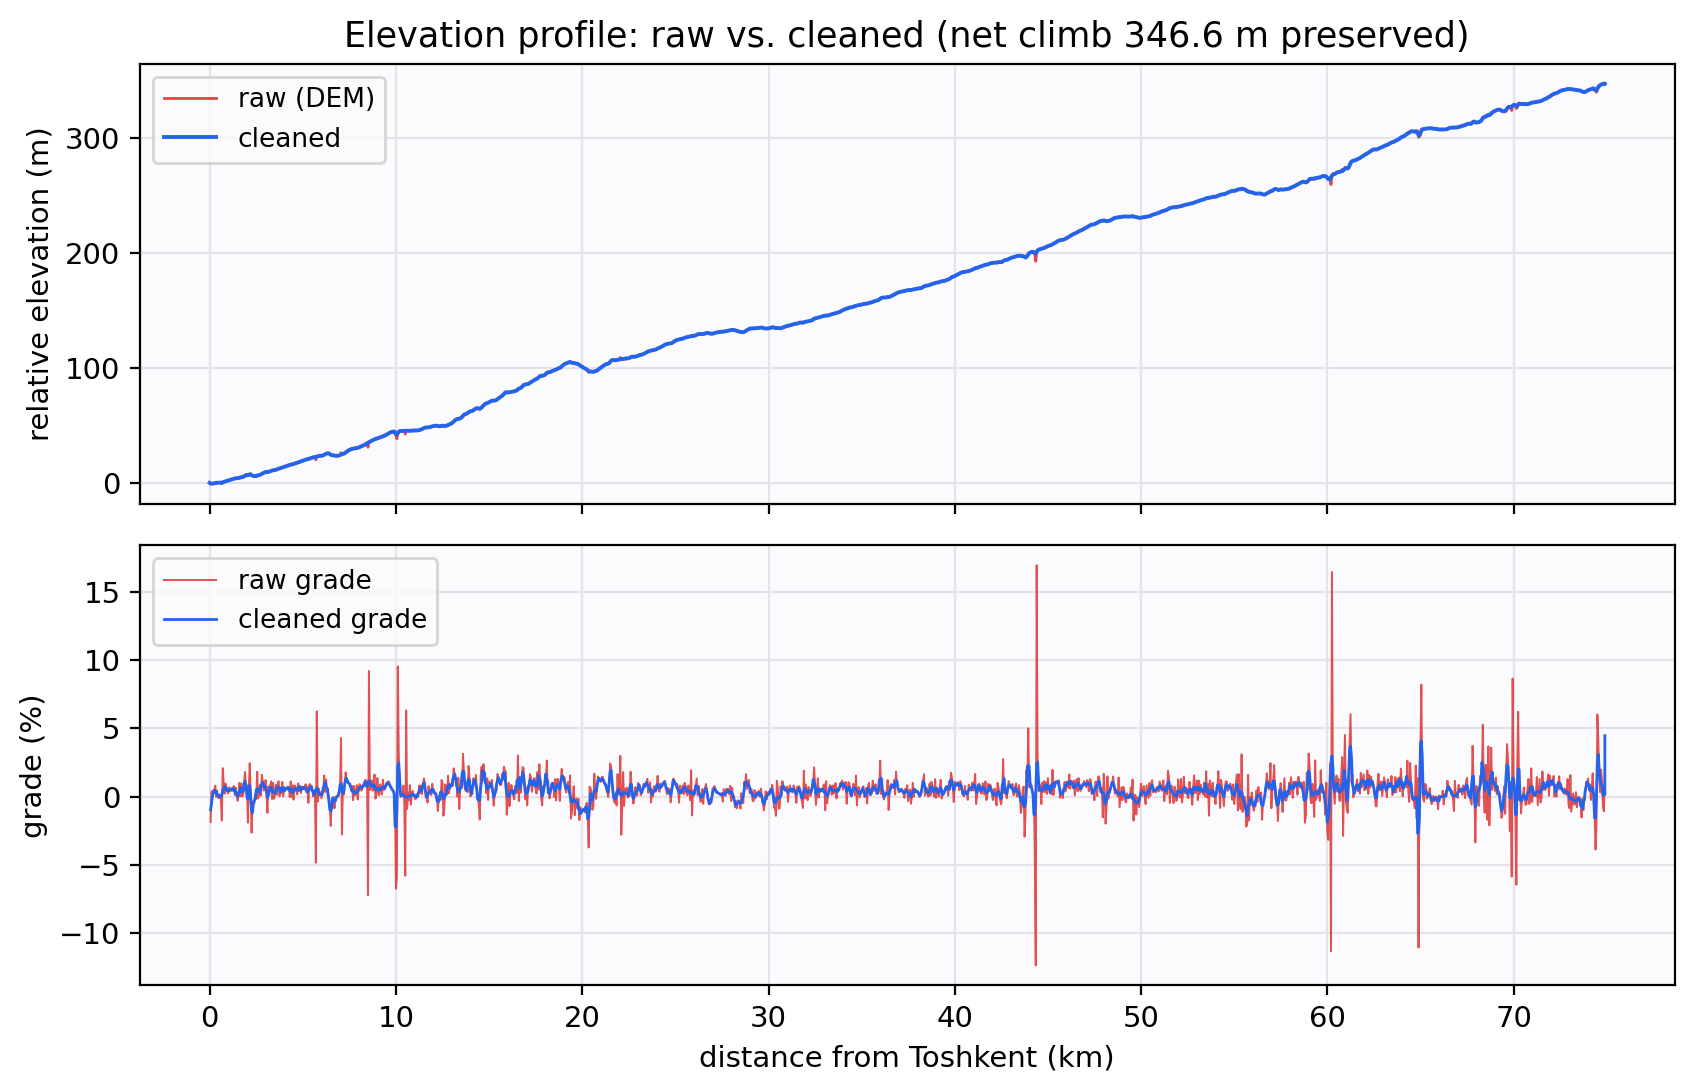
\includegraphics[width=.92\linewidth]{fig_data_cleaning.png}
\caption{Repair of the elevation noise. Top: elevation profile integrated
from the raw grades (red) and after median filtering (blue); the
endpoints are pinned, so the net climb of 346.6\,m is preserved exactly.
Bottom: the corresponding grade sequences. The raw spikes reach
$\pm$12--17\% on 50\,m segments, which no real railway exhibits and which
the simulator's force balance cannot absorb.}
\label{fig:cleaning}
\end{figure}

\subsection{Markov decision process formulation}
\label{sec:mdp}

\paragraph{Observation (9 features, all normalized).} Speed $v/22.22$,
position $x/L$, directional grade $i/4.5$, curvature, remaining distance
$(L-x)/L$, per-step energy $E_t/1.5$, link speed limit $v_{\lim}/22.22$,
elapsed-time fraction $\tau = t/T_d$, and the behind-schedule fraction
\begin{equation}
\beta_t \;=\; \max\!\Bigl(0,\ \tfrac{t}{T_d}L - x_t\Bigr)\big/ L .
\end{equation}
The last two features are not decoration. The reward below depends on the
step counter, and an agent with no clock among its observations faces a
reward it cannot predict from what it sees; Section~\ref{sec:results}
shows what that does in practice. The normalization denominators matter
just as much. Earlier values, calibrated to a previous dataset, clipped
the grade feature to a sign bit on 27\% of the route and saturated the
energy feature at 17\% of its true range. The agent was blind to exactly
the terrain and power information that terrain-aware driving needs.

\paragraph{Action.} One of nine notch settings, held for 15 consecutive
simulator seconds (action repeat). This cuts the decision horizon from
roughly 6{,}500 one-second choices per episode to roughly 430. We found
the reduction necessary for credit assignment over a trip-length energy
sum. With one-second decisions, every reward design we tried collapsed to
a near-constant notch.

\paragraph{Reward.} Per simulated second $t$, summed over the 15\,s
decision, with the smoothness term charged once per decision:
\begin{equation}
r_t \;=\; -\,w_E\, E_t \;-\; w_P\, \beta_t \;-\; w_V \max(0,\, v_t - v_{\lim})
\;\;\underbrace{-\; w_S\, |\Delta u|}_{\text{per decision}}
\;+\;
\begin{cases}
+B_{\mathrm{arr}} & \text{on arrival},\\[2pt]
-B_{\mathrm{to}} & \text{on timeout},
\end{cases}
\label{eq:reward}
\end{equation}
with $w_E{=}3$ per kWh, $w_P{=}2$, $w_V{=}1$, $w_S{=}0.15$,
$B_{\mathrm{arr}}{=}200$, $B_{\mathrm{to}}{=}1500$, and a timeout at
12{,}000\,s. The pace penalty $w_P \beta_t$ vanishes whenever the train
is on or ahead of the uniform deadline pace. Coasting is therefore free
wherever slack exists, and falling behind is charged immediately. We
tried a terminal-only lateness fee first; it does not work here. Over an
episode of some 6{,}000 steps, an energy saving collected now outweighs
any end-of-trip penalty of practical size once discounting is applied.

\paragraph{Near-undiscounted objective.} The quantity we care about is a
sum of energy over roughly 6{,}000 steps. With $\gamma \le 0.999$ the
discounting itself biases that sum toward early arrival, which means high
notch. We therefore use $\gamma = 0.9999$, giving an effective horizon
near $10^4$ steps, together with return normalization to keep the value
function stable.

\subsection{Learning setup}
\label{sec:learning}

\begin{table}[t]
\centering\small
\begin{threeparttable}
\caption{PPO hyperparameters (Tianshou 0.5.1~\cite{weng2022tianshou},
Gymnasium environment~\cite{towers2024gymnasium}).}
\label{tab:hyper}
\begin{tabular}{llll}
\toprule
Algorithm & PPO~\cite{schulman2017ppo}, separate actor/critic & Discount $\gamma$ & 0.9999 \\
Networks & MLP $[256,128,64]$ & GAE $\lambda$~\cite{schulman2016gae} & 0.95 \\
Optimizer & Adam, lr $3\times10^{-4}$ & Clip $\epsilon$ & 0.2 \\
Parallel envs & 8 (one C++ process each) & Value coef.\ / grad clip & 0.5 / 0.5 \\
Batch / reuse & 2048 / 4 epochs per collect & Adv.\ + return norm. & on / on \\
Episodes per collect & 8 (full episodes) & Entropy coef. & $0.004 \to 0$ linearly by ep.\ 140 \\
Budget & 200 epochs ($\approx$1{,}600 episodes, $\sim$37\,min)\tnote{a} & Checkpointing & best test reward \\
\bottomrule
\end{tabular}
\begin{tablenotes}\footnotesize
\item[a] Wall-clock time on the training workstation.
% TODO(author): state CPU/GPU specification (e.g. cores, GPU model) so
% the timing figure is reproducible.
\end{tablenotes}
\end{threeparttable}
\end{table}

Table~\ref{tab:hyper} lists the final configuration. One choice needs
explaining: the annealed entropy coefficient. With the coefficient held
constant at 0.004, the policy sat at the uniform distribution for the
full 100 epochs of run~A. Its entropy stayed at $\ln 9 = 2.197$, the
action histogram stayed flat, and the argmax parked at notch~0 and timed
out. The reason is a mismatch of gradient magnitudes. A single 15-second
notch choice moves an episode return of around 2{,}500 units only
slightly, so the per-decision advantage gradient is small, and the
entropy gradient beat it. Annealing the coefficient linearly to zero
keeps the early exploration but lets the policy commit later. Entropy
then falls (to 1.24 on the forward trip and 0.33 on the return at 200
epochs) and the test reward improves monotonically
(Figure~\ref{fig:training}).

% =====================================================================
\section{Results}
\label{sec:results}
% =====================================================================

\subsection{Constant-notch frontiers and built-in driver}

\begin{table}[t]
\centering\small
\begin{threeparttable}
\caption{Constant-notch baselines on the repaired data, measured through
the interactive simulator. Bold marks the lowest-energy schedule-feasible
constant policy (the ``eco target'') in each direction. The native
NeTrainSim driver was measured on the forward trip.}
\label{tab:frontier}
\begin{tabular}{l rr c rr}
\toprule
& \multicolumn{2}{c}{Forward (climb $+347$\,m)} & \hspace{4mm} & \multicolumn{2}{c}{Return (descent $-347$\,m)} \\
\cmidrule{2-3}\cmidrule{5-6}
Notch\tnote{a} & Time (s) & Energy (kWh) & & Time (s) & Energy (kWh) \\
\midrule
8 & 5{,}602 & 862.4 & & 5{,}605 & 348.3 \\
6 & 5{,}652 & 853.5 & & 5{,}641 & 335.8 \\
5 & 5{,}721 & 849.1 & & 5{,}682 & 327.4 \\
4 & 5{,}910 & 834.4 & & 5{,}768 & 317.7 \\
3 & \textbf{6{,}442} & \textbf{788.6} & & 5{,}950 & 293.9 \\
2 & 8{,}492\tnote{b} & 758.4 & & \textbf{6{,}375} & \textbf{242.2} \\
1 & --- & --- & & 7{,}681\tnote{b} & 170.1 \\
\midrule
Native driver & 6{,}038 & 848.2 & & --- & --- \\
\bottomrule
\end{tabular}
\begin{tablenotes}\footnotesize
\item[a] Notch 0 does not move the train and is omitted. Notch 1 does not
complete the climbing direction within the 12{,}000\,s timeout.
% TODO(author): notch 7 is missing from both columns -- either add the
% measurement or state in one sentence why it was not run.
\item[b] Misses the 6{,}500\,s deadline.
\end{tablenotes}
\end{threeparttable}
\end{table}

Table~\ref{tab:frontier} gives the energy--time Pareto frontiers obtained
by driving each constant notch to completion. Three properties of these
baselines matter later. The frontier is shallow at the top and steep at
the bottom: dropping from notch 8 to notch 4 on the forward trip buys
only 28\kwh{} for 308\,s of extra travel time, while the single step from
notch 4 to notch 3 buys 46\kwh{} for another 532\,s. The 6{,}500\,s
deadline makes constant notch~3 the eco target on the climb and notch~2
on the descent; these are the slowest constant policies that still arrive
on time. Finally, NeTrainSim's own driver, which varies the notch along
the route, lands \emph{above} the frontier, at 848.2\kwh{} in 6{,}038\,s,
which is more energy than constant notch~4 spends at a comparable time.
Varying the notch is evidently not better driving by itself.

\subsection{The diagnostic chain}

Table~\ref{tab:runs} summarizes the training runs. Beyond the data fault
repaired in Section~\ref{sec:data}, three more failure modes had to be
found and removed during training before anything was learned. We
document each because the symptoms are not specific to this project; any
long-horizon, simulator-in-the-loop RL setup can produce them.

\begin{table}[t]
\centering\small
\begin{threeparttable}
\caption{Training-run summary (all on repaired data, 9-feature
observation). ``Sampled'' rollouts draw from the policy distribution,
which is the behavior the test rewards measure; ``argmax'' is the
deterministic mode of the policy.}
\label{tab:runs}
\begin{tabular}{lllll}
\toprule
Run & Best reward & Sampled rollout & Argmax rollout & Diagnosis \\
\midrule
\multicolumn{5}{l}{\emph{Forward trip}} \\
A\enspace(100 epochs, constant entropy) & $-2470$ & uniform histogram & notch 0, timeout & entropy pinned at $\ln 9$ \\
B\enspace(100 epochs, annealed) & $-2323$ & 800.2\kwh, 6{,}708\,s & constant notch 2, 31\% late & sharp but late \\
C\enspace(200 epochs, annealed) & $-2254$ & \textbf{790.0\kwh, 6{,}417\,s} & constant notch 1, timeout & \textbf{frontier parity} \\
\midrule
\multicolumn{5}{l}{\emph{Return trip}} \\
D\enspace(100 epochs, annealed) & $-906$ & 319.7\kwh, 5{,}827\,s & constant notch 4, on time & still descending \\
E\enspace(200 epochs, annealed) & $-620$ & 169.6\kwh, 7{,}076\,s & constant notch 1, 18\% late & overshot deadline \\
\bottomrule
\end{tabular}
\end{threeparttable}
\end{table}

\paragraph{(i) Observation saturation.} Before the audits reported here,
the grade feature was normalized by a constant of $0.7\%$ left over from
an earlier dataset. Against the real cleaned grades of up to $\pm4.5\%$,
the feature clipped to $\pm1$ on 27\% of the route. A 1\% climb and a 4\%
climb looked identical to the policy. The per-step energy feature had the
same problem, saturating at 0.25\kwh{} against a true maximum of
1.39\kwh. No terrain-aware policy can be learned by an agent that cannot
see terrain magnitude. We would add that conclusions about what RL
``cannot do'' on a problem are worth little until such an audit has been
run.

\paragraph{(ii) Non-Markovian reward.} The pace penalty in
Eq.~\eqref{eq:reward} depends on the elapsed step count, which the
observation originally did not contain. The critic was being asked to
predict targets from inputs that do not determine them, and the policy
had no way to condition on schedule slack, which is exactly the
capability the problem calls for. Adding $\tau$ and $\beta$ to the
observation restored the Markov property and the problem disappeared.

\paragraph{(iii) Exploration--commitment deadlock.} Run~A in
Table~\ref{tab:runs}. Under the constant entropy bonus the policy stayed
exactly uniform for 100 epochs while still collecting a reward of
$-2470$, because uniformly random notches happen to average out to a
feasible pace. The sampled behavior masked the defect entirely. What
exposed it was the argmax, which sat at notch 0 and timed out, together
with the entropy trace. Switching to linear annealing
(Section~\ref{sec:learning}) broke the deadlock without giving up early
exploration; run~B improved the best reward by 147 units and produced the
first sharp, usable policy.

\begin{figure}[t]
\centering
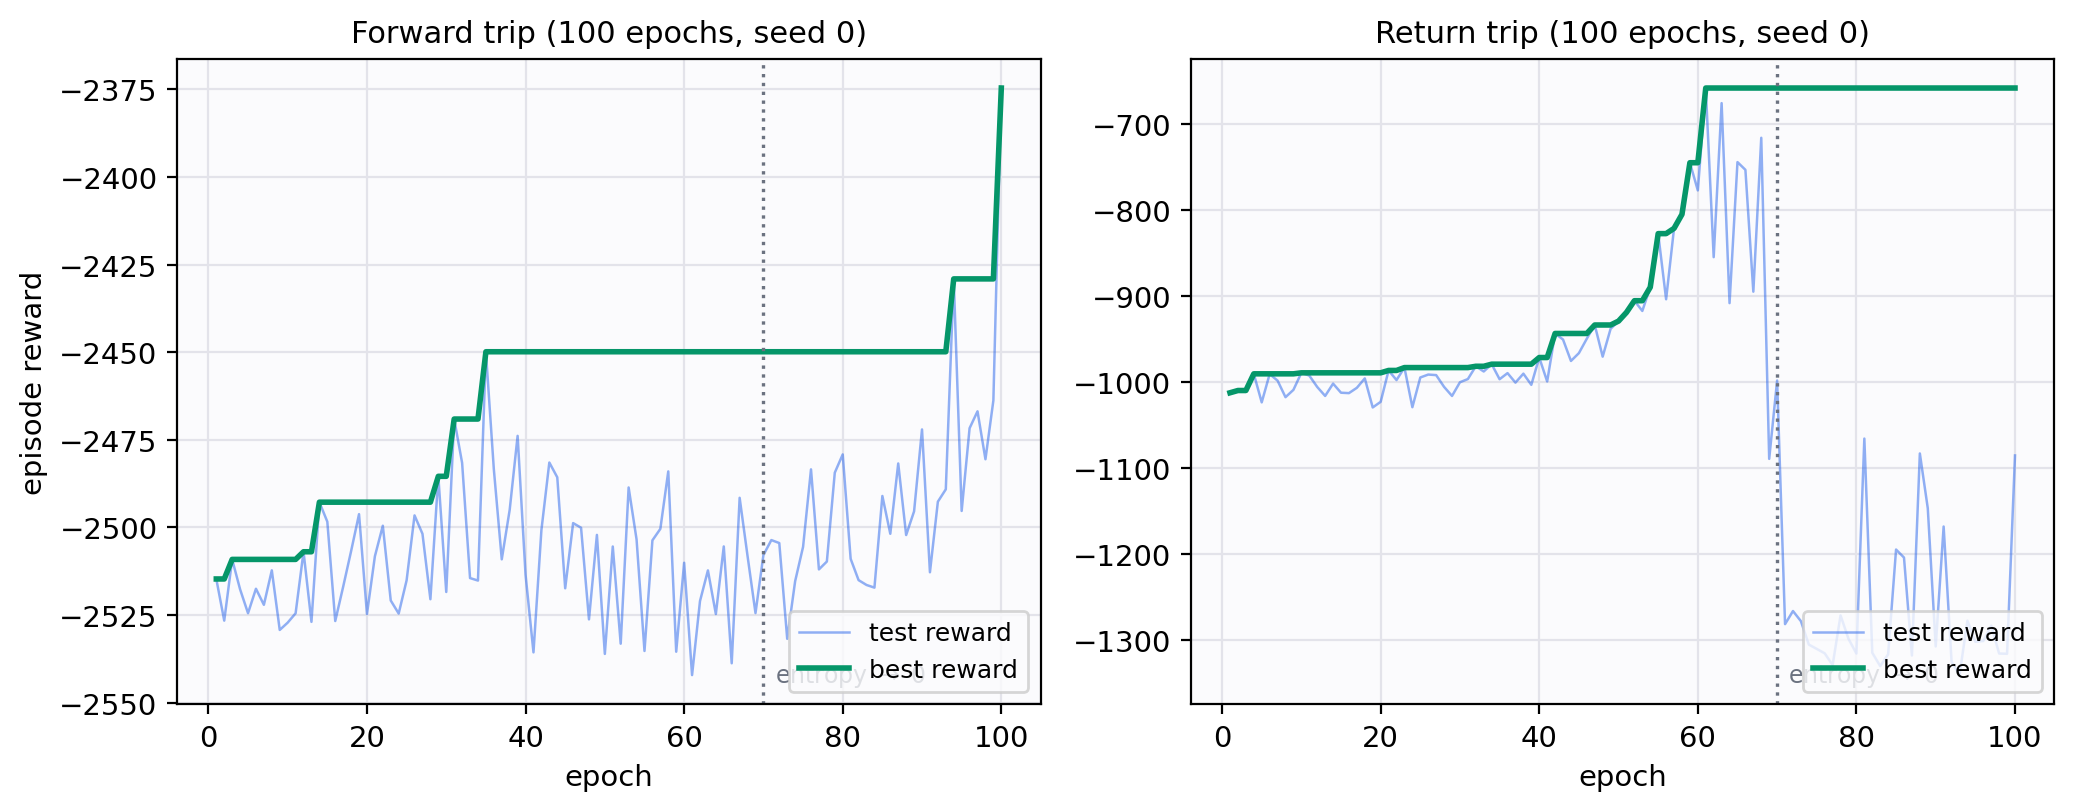
\includegraphics[width=.95\linewidth]{fig_training_curves.png}
\caption{Training curves for the 200-epoch runs (left: forward; right:
return). Test rewards are single sampled episodes; the dotted line marks
the epoch at which the entropy coefficient reaches zero. Both runs keep
improving through the annealed phase. The forward run peaks at $-2254$
(epoch 196), the return run at $-620$ (epoch 179).}
\label{fig:training}
\end{figure}

\subsection{Forward trip: on-schedule frontier parity}

\begin{figure}[t]
\centering
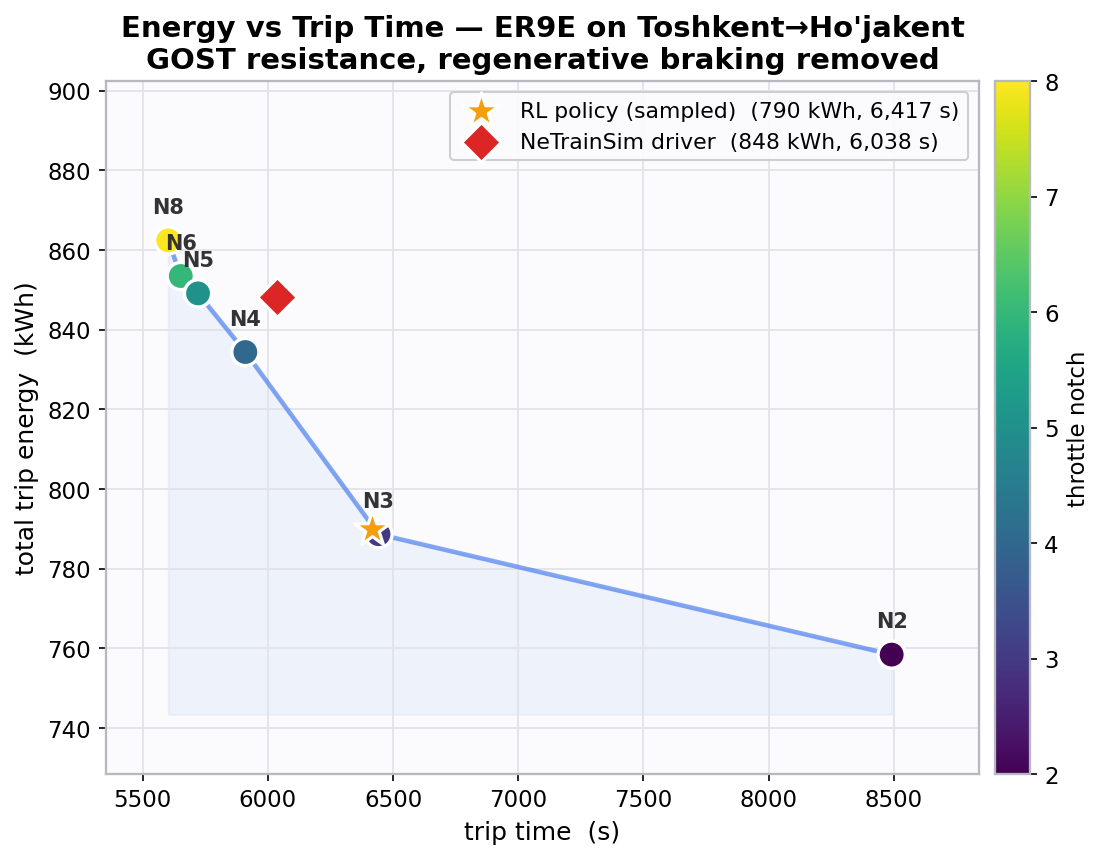
\includegraphics[width=.8\linewidth]{fig_tradeoff_forward.png}
\caption{Forward trip: constant-notch frontier (colored by notch), the
native NeTrainSim driver (red diamond), and the learned sampled policy
(orange star) at 790.0\kwh{} / 6{,}417\,s, on schedule and within about
1\kwh{} of the interpolated frontier.}
\label{fig:tradeoff_fwd}
\end{figure}

\begin{figure}[t]
\centering
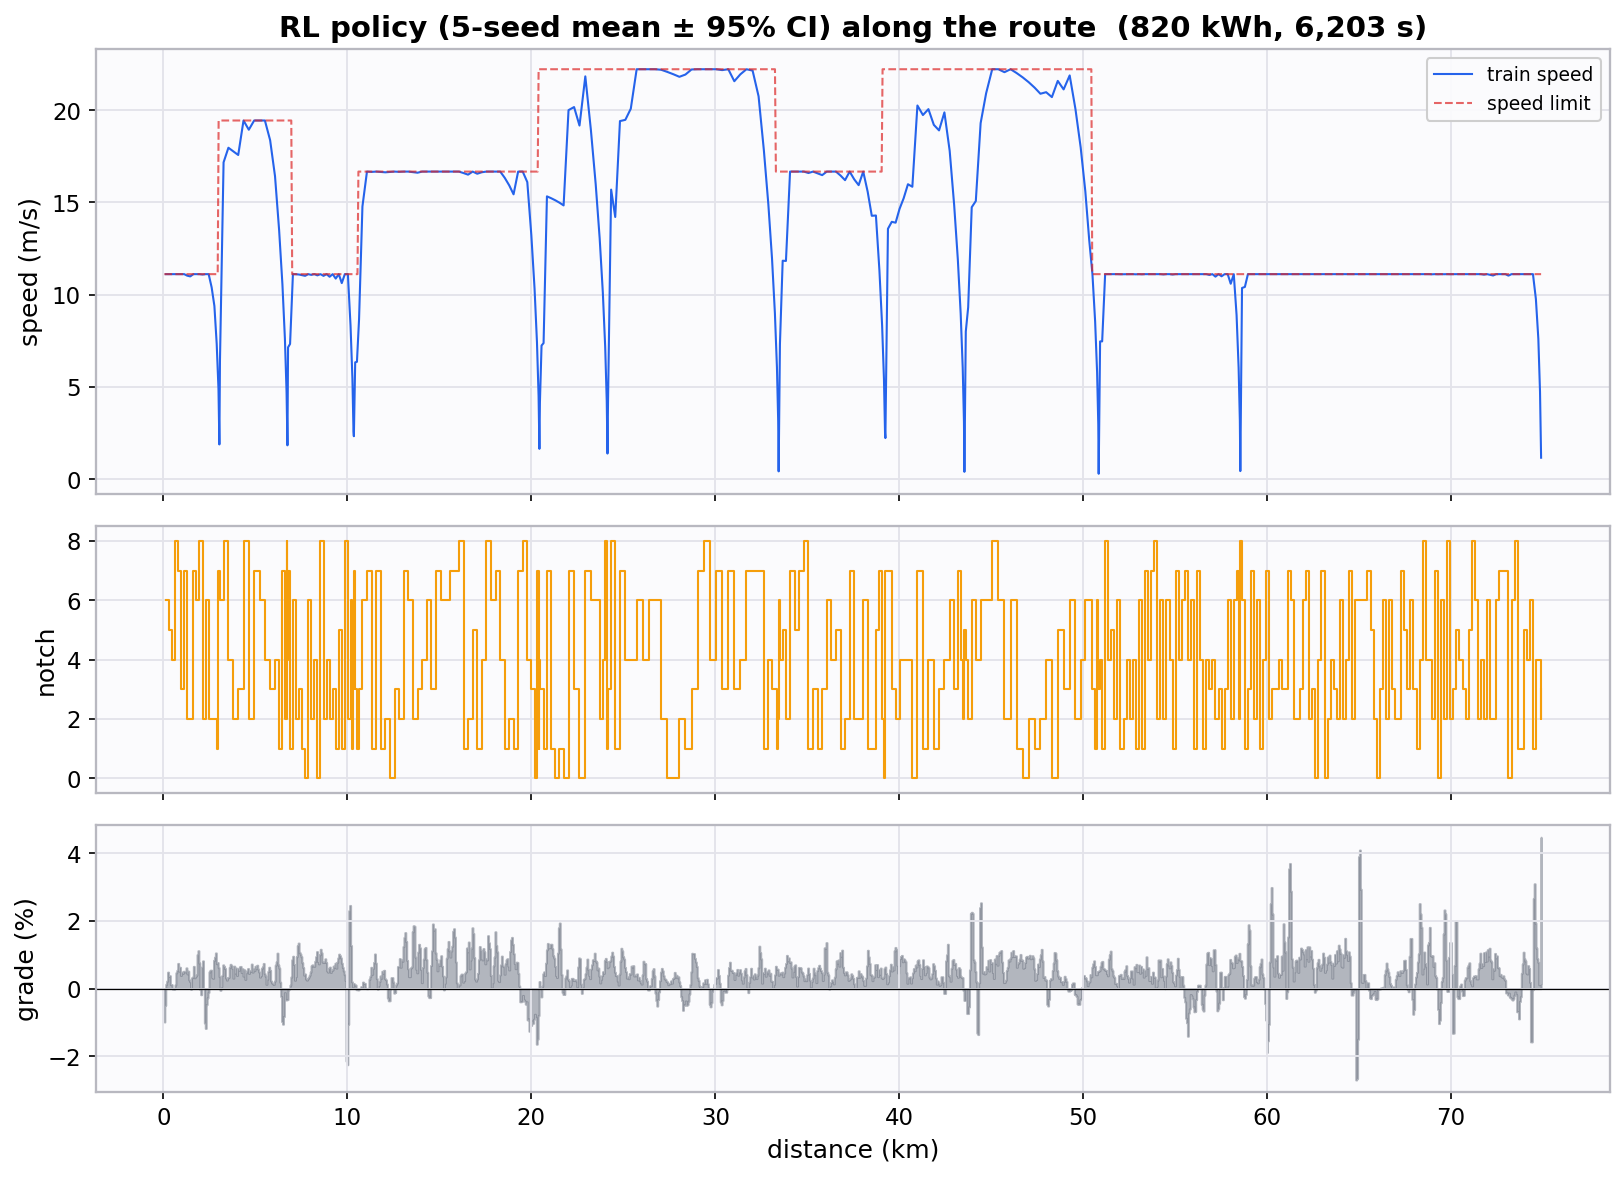
\includegraphics[width=.9\linewidth]{fig_profile_forward.png}
\caption{Learned forward policy (sampled) along the route: speed against
the limit, notch sequence, and gradient. The policy idles at low notch
and inserts short higher-notch efforts to hold deadline pace.}
\label{fig:profile_fwd}
\end{figure}

The 200-epoch forward policy (run~C) reaches 790.0\kwh{} in 6{,}417\,s
when sampled, which is 83\,s inside the deadline. Interpolating the
constant-notch frontier linearly at 6{,}417\,s gives 790.8\kwh, so the
learned policy sits on the frontier to within measurement noise
(Figure~\ref{fig:tradeoff_fwd}). Against the fixed references, that is
8.4\% less energy than maximum-notch driving (notch 8, 862.4\kwh) and
6.9\% less than the simulator's native driver (848.2\kwh), with the
schedule met. The notch profile in Figure~\ref{fig:profile_fwd} shows a
low-notch base with selective bursts, which fits the shape of the
frontier: with a shallow top and a steep bottom, the cheap strategy is to
spend time at low notch and buy back pace in short, efficient efforts.

Two caveats. The policy matches the frontier but does not go below it. On
this route, with this resistance model, modulating the notch within the
trip seems to offer little energy beyond what the right constant notch
already captures, and the native varied-notch driver sitting above the
frontier points the same way. Second, the deterministic argmax of run~C
collapses to constant notch~1 and times out. The sampled policy is the
deployable artifact; the argmax pathology is taken up next.

\subsection{Return trip and the lateness-pricing defect}

\begin{figure}[t]
\centering
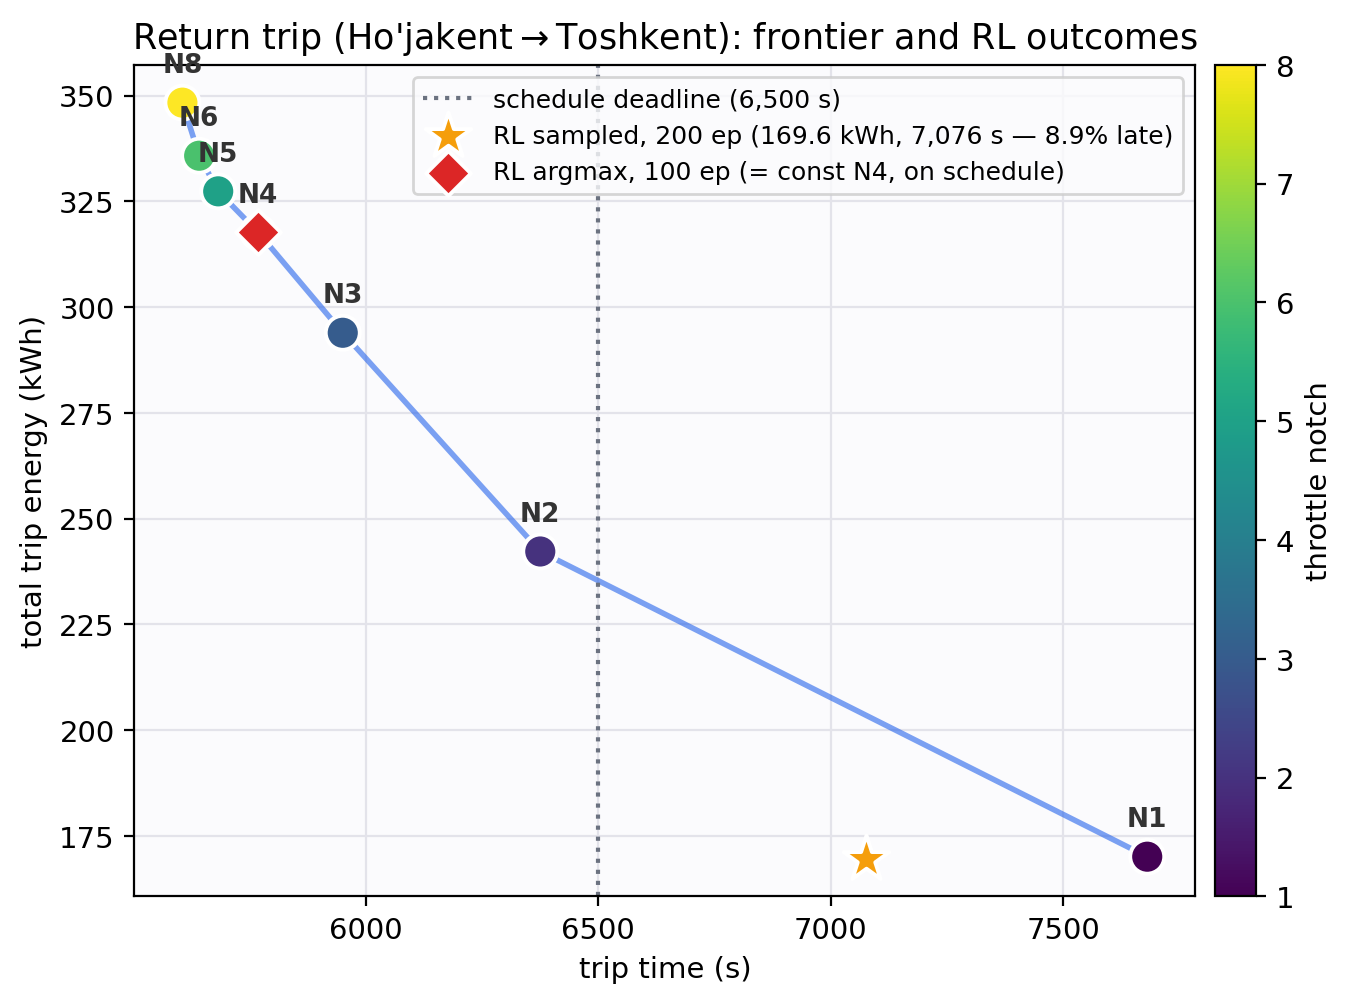
\includegraphics[width=.8\linewidth]{fig_tradeoff_return.png}
\caption{Return trip: frontier, deadline, and RL outcomes. The 100-epoch
argmax (red diamond) lands exactly on constant notch 4, on schedule. The
200-epoch sampled policy (orange star) descends past the eco point into
cheap-but-late territory (169.6\kwh, 8.9\% late).}
\label{fig:tradeoff_ret}
\end{figure}

\begin{figure}[t]
\centering
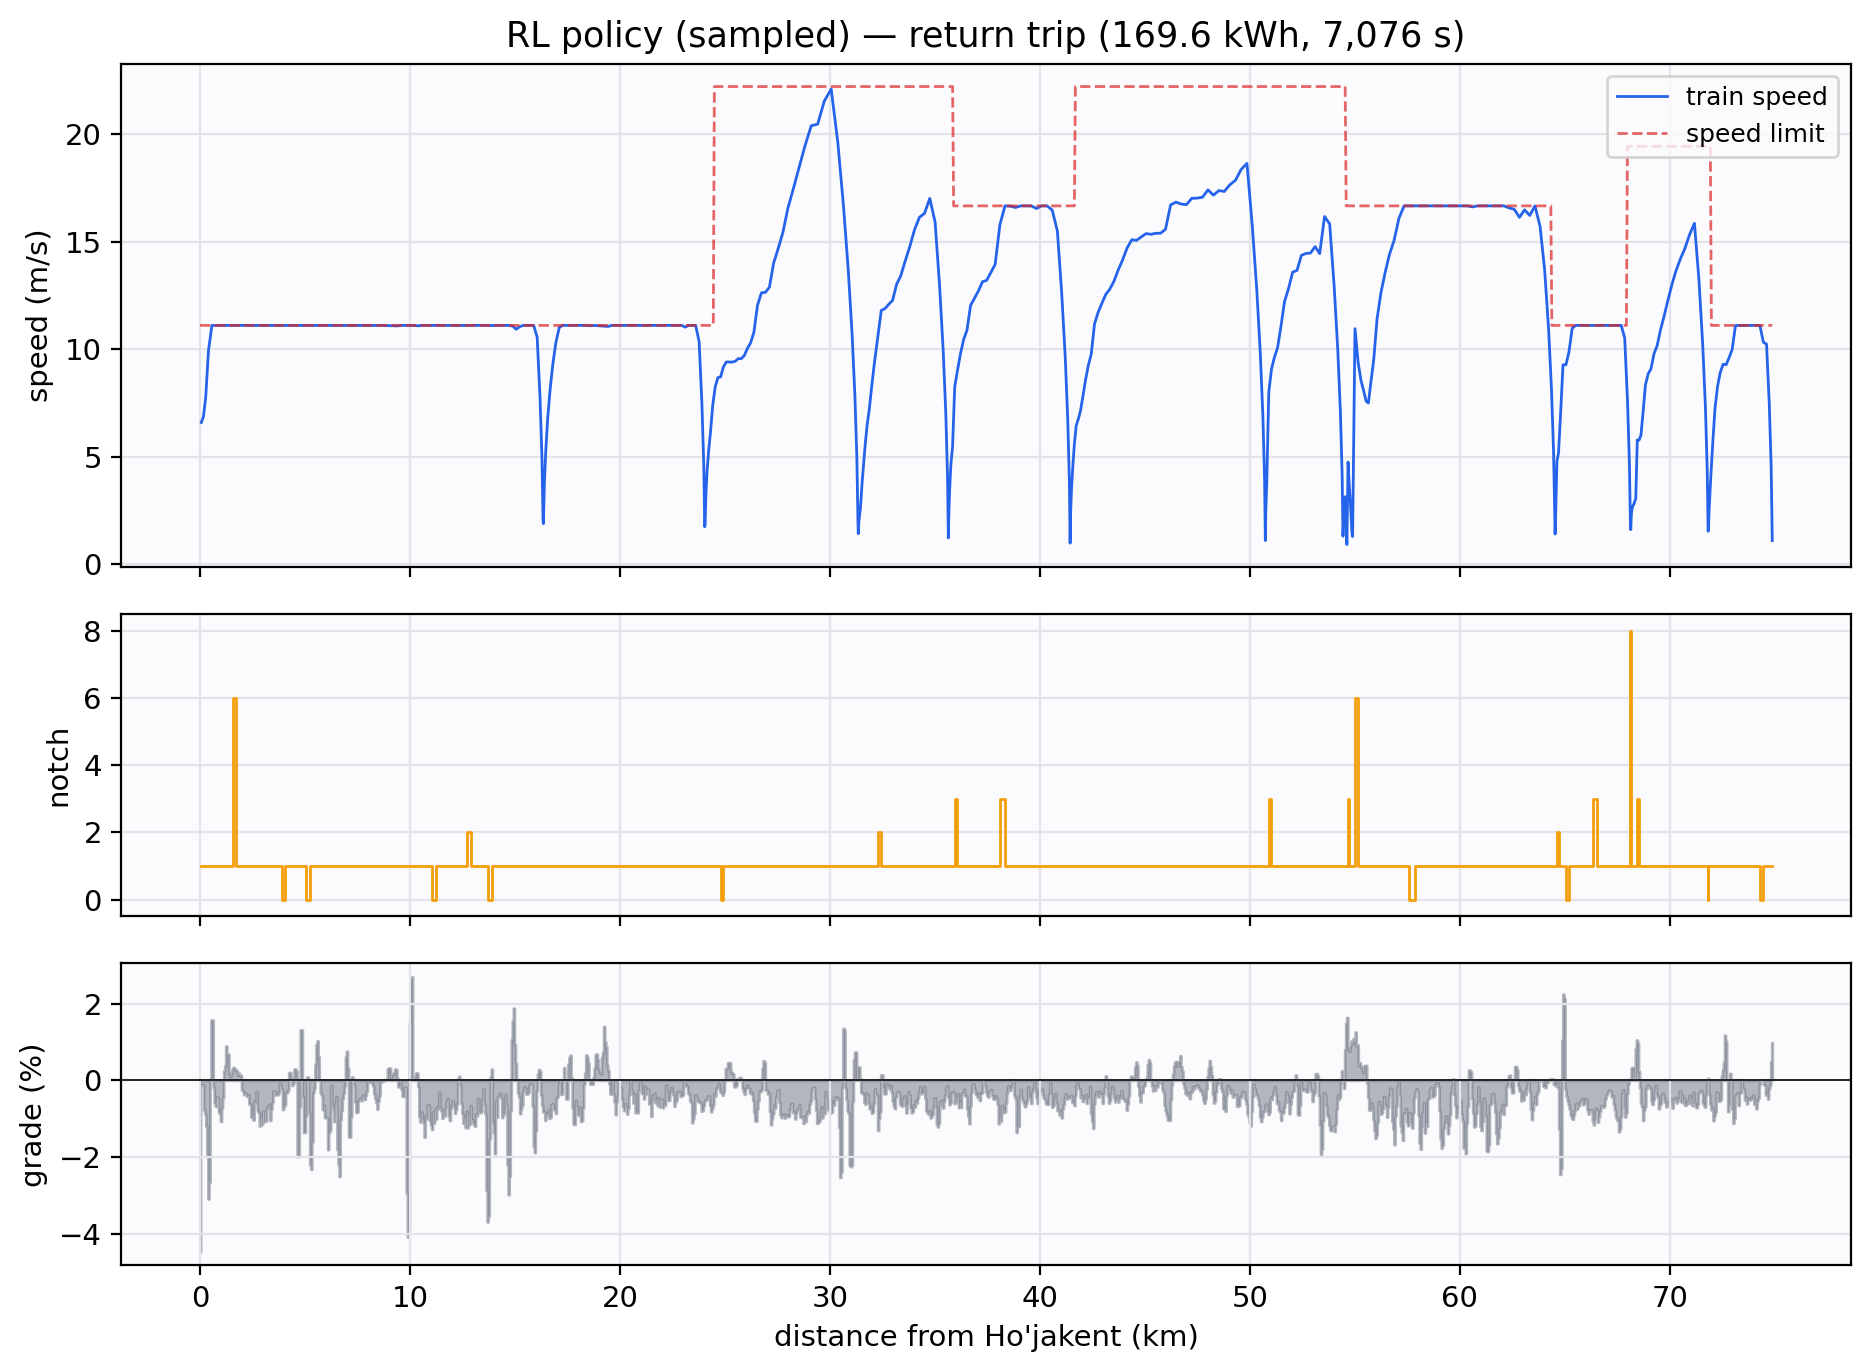
\includegraphics[width=.9\linewidth]{fig_profile_return.png}
\caption{Return-trip sampled policy: near-constant notch 1 with sparse
corrective bursts on the $-347$\,m net descent.}
\label{fig:profile_ret}
\end{figure}

The descending return trip is far cheaper everywhere
(Table~\ref{tab:frontier}), and its eco target is constant notch~2 at
242.2\kwh{} in 6{,}375\,s. At 100 epochs (run~D) the argmax is a clean,
on-schedule constant notch~4 at 317.7\kwh. That is the correct side of
the deadline, two notches above the optimum, and the run was still
improving when the budget ran out. So we doubled the budget. Run~E
continued the descent, but past the eco point: the sampled policy settles
at near-constant notch~1 (Figure~\ref{fig:profile_ret}), spends only
169.6\kwh, and arrives 576\,s late, an 8.9\% deadline violation. The
argmax is constant notch~1 at 18\% late (Figure~\ref{fig:tradeoff_ret}).

The optimizer is not at fault here. Reward rose monotonically and the
policy is sharp. The fault is in the prices in Eq.~\eqref{eq:reward}.
Going one notch below the eco point saves about 72\kwh{} on the return
trip, which is 216 reward units at $w_E{=}3$, while the pace penalty this
incurs at $w_P{=}2$ is of comparable size. The reward's optimum therefore
sits slightly below deadline pace even though the intended optimum sits
on it. The same arithmetic explains every argmax pathology in
Table~\ref{tab:runs}: the mode of the policy settles at the energy floor
of the reward-viable region, one notch under schedule-feasible, and
sampling noise supplies the missing pace. The fix is a calibration, not a
redesign. Raise $w_P$ until the marginal lateness cost strictly dominates
the marginal one-notch energy saving on both trips, which the arithmetic
above puts at $w_P \gtrsim 4$--$6$, or make the deadline a hard
constraint, for instance a large terminal penalty scaled by lateness on
top of the per-step pace term. We leave the $w_P$ ablation to future work
(Section~\ref{sec:conclusion}).

% =====================================================================
\section{Discussion and Limitations}
\label{sec:discussion}
% =====================================================================

\paragraph{What transfers.} None of the failure modes in this paper is
about trains. Data artifacts that quietly break simulator physics,
normalization constants that drift out of date, schedule rewards with no
clock in the observation, entropy bonuses that overpower weak
per-decision advantages, constraints priced below the savings they are
meant to block: any long-horizon RL project that runs through a simulator
on hand-maintained input data is exposed to all of them. Each one also
has a cheap, specific audit. Integrate and plot the derived physical
profiles. Histogram every observation feature against its bounds. Check
each reward term for dependence on state the observation does not carry.
Track policy entropy against $\ln |\mathcal{A}|$. And verify that the
optimum of the reward is the operating point you actually want.

\paragraph{Energy accounting under force-balance violation.} NeTrainSim
charges energy from the virtual tractive power $(ma + R)v$. When bad data
pushes $R$ past the adhesion limit, the recorded power can exceed the
installed power several times over, as Section~\ref{sec:data} showed.
After the repair, the largest per-step energy (1.39\kwh, a 5.0\,MW draw)
is consistent with the installed traction power once drivetrain losses
are counted. Any simulation study that totals energy over a route without
auditing the grade data first inherits this risk.

\paragraph{Limitations.} The results are single-route, single-consist,
and entirely in-simulator; we claim no field validation. The unit of the
curvature column is unverified (footnote in
Section~\ref{sec:simulator}), although the curve term is small under
either reading. The deterministic argmax is currently unusable on both
trips; we present sampled rollouts and have identified the calibration
cause. Regenerative braking is excluded by design for this stock, and on
a $-347$\,m descent regeneration would change the picture substantially.
Finally, the 15\,s action repeat that makes credit assignment tractable
also limits how finely the policy can modulate. Whether 1--5\,s control
with a hierarchical or reward-shaped scheme can get \emph{below} the
frontier is an open question.

% =====================================================================
\section{Conclusion}
\label{sec:conclusion}
% =====================================================================

We built and audited an end-to-end pipeline coupling PPO to a modified
NeTrainSim with true per-second throttle control, repaired the route data
the pipeline depends on, and trained driving policies for both directions
of the Tashkent--Khojikent line. The forward-trip policy reaches
on-schedule parity with the constant-notch Pareto frontier (790.0\kwh{}
in 6{,}417\,s; 8.4\% under maximum-notch driving and 6.9\% under the
simulator's native driver). The full diagnostic chain, from data repair
through observation audit, Markov repair, entropy annealing, and lateness
pricing, is documented with a measurement at every step. What remains
between the learned mode and the schedule-feasible optimum is a
one-parameter reward calibration whose arithmetic we have given, not an
open-ended search. We hope the study is useful beyond this particular
line, as a working checklist for anyone pushing long-horizon RL through
an imperfect simulator on imperfect data.

\paragraph{Future work.} Raise the lateness price $w_P$ and report
on-schedule convergence on both trips; run regeneration-capable stock on
the descending direction; probe for below-frontier terrain modulation
with finer control intervals and hierarchical policies; test robustness
to consist mass and timetable perturbations; and calibrate the GOST
coefficients and the curvature unit against field data.

% =====================================================================
\section*{Acknowledgments}
This work was supported by the Uzbekistan--China joint research grant
No.~IL-8724053120, ``Energy-saving technology for urban railway systems.''
% TODO(author): add supervisor/collaborators and any second funding line
% as appropriate before submission.

\section*{Declarations}
\paragraph{Conflict of interest.} The authors declare no conflict of
interest.
\paragraph{Data availability.} The modified NeTrainSim source code, the
repaired route dataset, and the training scripts are available from the
authors upon reasonable request.
% TODO(author): replace with a public repository link (e.g. GitHub/Zenodo)
% if/when the code is released. Many target journals now require this.

% =====================================================================
\begin{thebibliography}{13}\small

\bibitem{scheepmaker2017}
G.~M. Scheepmaker, R.~M.~P. Goverde, and L.~G. Kroon,
``Review of energy-efficient train control and timetabling,''
\emph{European Journal of Operational Research}, vol.~257, no.~2,
pp.~355--376, 2017.

\bibitem{howlett1995}
P.~G. Howlett and P.~J. Pudney,
\emph{Energy-Efficient Train Control}.
Springer-Verlag, London, 1995.

\bibitem{liu2003}
R.~Liu and I.~M. Golovitcher,
``Energy-efficient operation of rail vehicles,''
\emph{Transportation Research Part A: Policy and Practice}, vol.~37,
no.~10, pp.~917--932, 2003.

\bibitem{albrecht2016}
A.~Albrecht, P.~Howlett, P.~Pudney, X.~Vu, and P.~Zhou,
``The key principles of optimal train control---Part 1: Formulation of the
model, strategies of optimal type, evolutionary lines, location of optimal
switching points,''
\emph{Transportation Research Part B: Methodological}, vol.~94,
pp.~482--508, 2016.

\bibitem{yin2017}
J.~Yin, T.~Tang, L.~Yang, J.~Xun, Y.~Huang, and Z.~Gao,
``Research and development of automatic train operation for railway
transportation systems: A survey,''
\emph{Transportation Research Part C: Emerging Technologies}, vol.~85,
pp.~548--572, 2017.

\bibitem{yin2014}
J.~Yin, D.~Chen, and L.~Li,
``Intelligent train operation algorithms for subway by expert system and
reinforcement learning,''
\emph{IEEE Transactions on Intelligent Transportation Systems}, vol.~15,
no.~6, pp.~2561--2571, 2014.

\bibitem{mnih2015}
V.~Mnih \emph{et al.},
``Human-level control through deep reinforcement learning,''
\emph{Nature}, vol.~518, no.~7540, pp.~529--533, 2015.

\bibitem{aredah2024}
A.~S. Aredah, K.~Fadhloun, and H.~A. Rakha,
``NeTrainSim: a network-level simulator for modeling freight train
longitudinal motion and energy consumption,''
\emph{Railway Engineering Science}, vol.~32, pp.~480--498, 2024.
doi: 10.1007/s40534-024-00331-x.

\bibitem{schulman2017ppo}
J.~Schulman, F.~Wolski, P.~Dhariwal, A.~Radford, and O.~Klimov,
``Proximal policy optimization algorithms,''
arXiv preprint arXiv:1707.06347, 2017.

\bibitem{schulman2016gae}
J.~Schulman, P.~Moritz, S.~Levine, M.~Jordan, and P.~Abbeel,
``High-dimensional continuous control using generalized advantage
estimation,'' in \emph{Proceedings of the International Conference on
Learning Representations (ICLR)}, 2016.

\bibitem{weng2022tianshou}
J.~Weng, H.~Chen, D.~Yan, K.~You, A.~Duburcq, M.~Zhang, Y.~Su, H.~Su, and
J.~Zhu, ``Tianshou: A highly modularized deep reinforcement learning
library,'' \emph{Journal of Machine Learning Research}, vol.~23, no.~267,
pp.~1--6, 2022.

\bibitem{towers2024gymnasium}
M.~Towers \emph{et al.},
``Gymnasium: A standard interface for reinforcement learning environments,''
arXiv preprint arXiv:2407.17032, 2024.

\bibitem{companion}
K.~Mustaev and A.~Boboyev,
``A calibrated longitudinal-dynamics and resistance model for legacy
1520\,mm-gauge electric multiple units: The ER9E on the
Tashkent--Khojikent corridor,'' manuscript in preparation, 2026.
% TODO(author): update status (submitted / under review / preprint DOI)
% before submission.

\end{thebibliography}

\end{document}
